\section{Introduction}
Signs like zebra crossing and barred area are multi contour. Detection of such signs are discussed in this chapter.

\section{Zebra crossing detection}
\begin{figure}[h!]
    \centering
    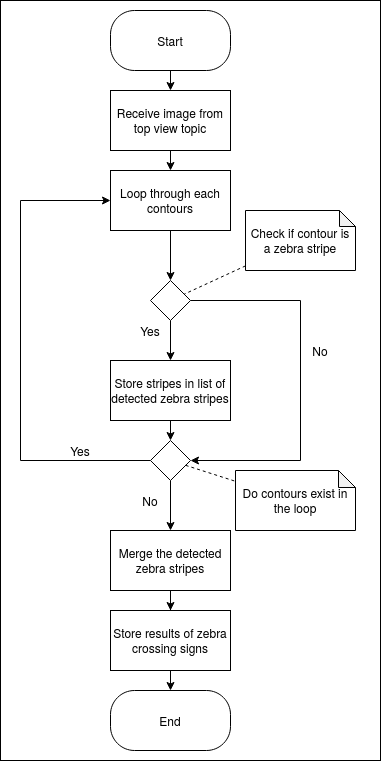
\includegraphics[scale=0.45]{images/ZebraCrossingFlowChart.png}
    \caption{Flow chart of detection of zebra crossing sign}
\end{figure}

Steps \textbf{``Receive image from top view topic''} and \textbf{`` Loop through each contours''} are already discussed in \autoref{subsec:RecieveImageFromTopView} and \autoref{subsec:LoopThroughContours}

\subsection{Check if contour is a zebra stripe}
\label{sec:ZebraCrossingStripeChecking}
From each contour a \href{https://docs.opencv.org/3.4.3/db/dd6/classcv_1_1RotatedRect.html}{\emph{cv::RotatedRect}} is extracted and it is checked whether it is a zebra stripe or not. This is done in \emph{ZebraCrossing::isRectZebraStripe()} function. Following are the lists of dimensional constants against which \href{https://docs.opencv.org/3.4.3/db/dd6/classcv_1_1RotatedRect.html}{\emph{cv::RotatedRect}} of the contour is checked for zebra stripe.
\begin{itemize}
    \item {\small \textbf{ZEBRA\_CROSSING\_MINIMUM\_HEIGHT}}
    \item {\small \textbf{ZEBRA\_CROSSING\_MAXIMUM\_HEIGHT}}
    \item {\small \textbf{ZEBRA\_CROSSING\_MINIMUM\_WIDTH}}
    \item {\small \textbf{ZEBRA\_CROSSING\_MAXIMUM\_WIDTH}}
\end{itemize}

\subsection{Store stripes in list of detected zebra stripes}
The contours which are detected as zebra stripe in previous step. Those \href{https://docs.opencv.org/3.4.3/db/dd6/classcv_1_1RotatedRect.html}{\emph{cv::RotatedRect}} are stored in a list for merging them together.

\subsection{Merge the detected zebra stripes}
The list of \href{https://docs.opencv.org/3.4.3/db/dd6/classcv_1_1RotatedRect.html}{\emph{cv::RotatedRect}} which are candidate zebra stripes are merged together using \emph{ZebraCrossing::clusterStripesForZebraCro-ssings()} function. This function then outputs the zebra crossing signs on the lane for a given frame.
\begin{figure}[ht]
\begin{subfigure}{0.5\textwidth}
\centering
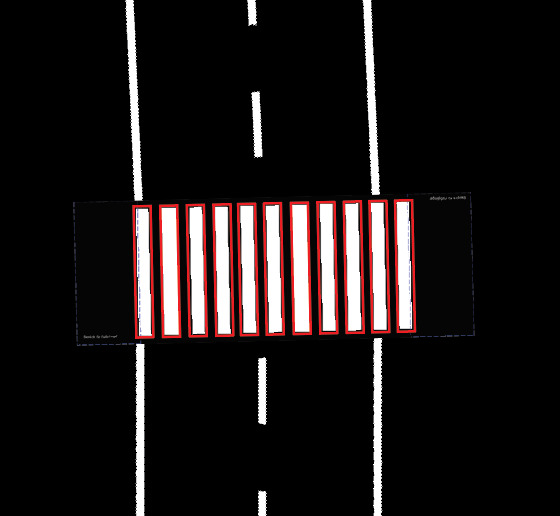
\includegraphics[width=0.9\linewidth,height=5cm]{images/UnmergedZebraStripes.jpeg} 
\caption{Before merging the zebra stripes}
\end{subfigure}
\begin{subfigure}{0.5\textwidth}
\centering
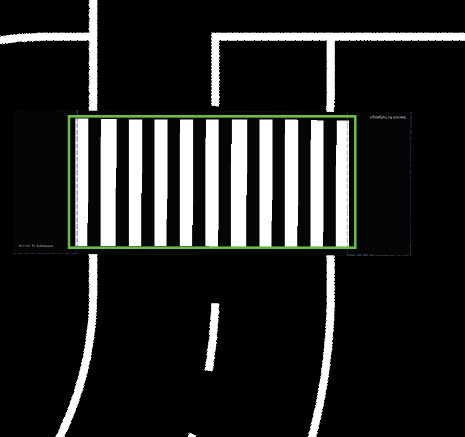
\includegraphics[width=0.9\linewidth,height=5cm]{images/MergedZebraStripes.jpeg} 
\caption{After merging the zebra stripes}
\end{subfigure}
\caption{Before and after merging the zebra stripes}
\label{fig:BeforeAfterMergingZebraStripes}
\end{figure}

\subsection{Store results of zebra crossing signs}
\label{sec:ZebraCrossStoreResults}
The zebra crossing signs which are detected in previous step are stored for publishing them as results. Details about how to publish are discussed in \autoref{chap:PublishResults}

\section{Barred area detection}
\begin{figure}[h]
    \centering
    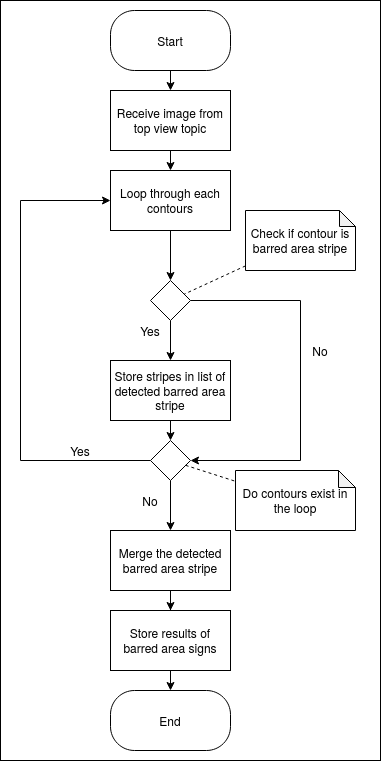
\includegraphics[scale=0.44]{images/BarredAreaFlowChart.png}
    \caption{Flow chart of detection of barred area sign}
\end{figure}

Steps \textbf{``Receive image from top view topic''} and \textbf{`` Loop through each contours''} are already discussed in \autoref{subsec:RecieveImageFromTopView} and \autoref{subsec:LoopThroughContours}

\subsection{Check if contour is a barred area stripe}
\label{sec:BarredAreaStripeChecking}
Each contour is checked whether it is a barred area stripe or not in \emph{BarredAreaStripe::isBarredAreaStripe()} function. Following are the list of dimensional constants against which the contour is checked for barred area stripe.
\begin{itemize}
    \item {\small \textbf{SMALLER\_SIDE\_MINIMUM\_LENGTH}}
    \item {\small \textbf{SMALLER\_SIDE\_MAXIMUM\_LENGTH}}
    \item {\small \textbf{LARGE\_SIDE\_MINIMUM\_LENGTH}}
    \item {\small \textbf{LARGE\_SIDE\_MAXIMUM\_LENGTH}}
    \item {\small \textbf{MIN\_ACUTE\_ANGLE}}
    \item {\small \textbf{MAX\_ACUTE\_ANGLE}}
    \item {\small \textbf{MIN\_OBTUSE\_ANGLE}}
    \item {\small \textbf{MAX\_OBTUSE\_ANGLE}}
\end{itemize}

\subsection{Store stripes in list of detected barred area stripes}
The stripes which are detected in previous step are stored in the list of \emph{BarredAreaStripe} type for merging them later.

\subsection{Merge the detected barred area stripes}
The list of \emph{BarredAreaStripe} type are merged together using \\\emph{BarredArea::clusterStripes()} function. This function outputs the barred area on the lane for a given frame.

\newpage

\begin{figure}[ht]
\begin{subfigure}{0.5\textwidth}
\centering
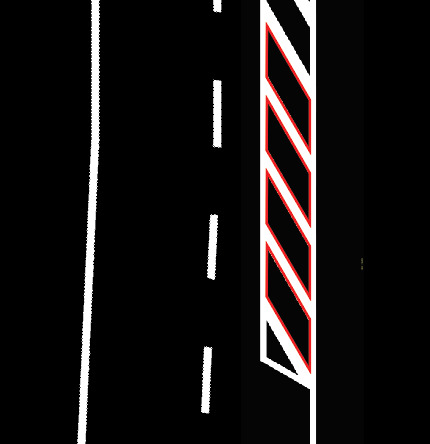
\includegraphics[width=0.9\linewidth,height=5cm]{images/UnmergedBarredAreaStripes.jpeg} 
\caption{Before merging the barred area stripes}
\end{subfigure}
\begin{subfigure}{0.5\textwidth}
\centering
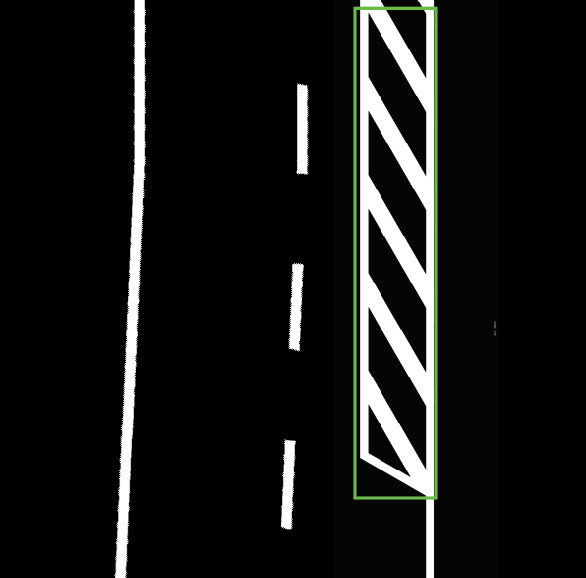
\includegraphics[width=0.9\linewidth,height=5cm]{images/MergedBarredAreaStripes.jpeg} 
\caption{After merging the barred area stripes}
\end{subfigure}
\caption{Before and after merging the barred area stripes}
\label{fig:BeforeAfterMergingBarredAreaStripes}
\end{figure}

\subsection{Store results of barred area signs}
\label{sec:BarredAreaStoreResults}
The barred area signs which are detected in previous tep are stored for publishing them as results. Details about how to publish are discussed in \autoref{chap:PublishResults}.